\documentclass[aspectratio=169]{beamer}
\usepackage[UKenglish]{babel}
\usepackage[T1]{fontenc} % fontenc mit T1 sorgt für richtige Kodierung europäischer Zeichen
\usepackage[utf8]{inputenc} % Eingabezeichensatz: direkte Eingabe von Umlauten usw.
 % Anpassung des Dokumants deutsche Richtlinien

\usepackage{url} %Einbinden von Hyperlinks
\usepackage{mdwlist} % Für Listen ohne Abstand zwischen den Aufzählungspunkten.
\usepackage{paralist} % Ermöglicht Anpassung der Listen, z.B. Wahl des Autfählungszeichens

\usepackage{setspace} % Anpassung des Zeilenabstandes, Befehl muss vor der Berechnung des Satzspiegels gesetzt werden.

\usepackage{varioref} %Querverweise mit Seitenreferenz
\usepackage{fancyref} %Querverweise mit Angabe des Typs
%\usepackage[table,gray]{xcolor} %Zum Deaktivieren von Schattierung -- nur bei Verwendung des Pakets "listings"
\usepackage{booktabs} %Zur eleganten Formatierung von Tabellen
\usepackage{tabularx}
\usepackage[format = plain, textfont = normalfont, labelfont = bf, font = scriptsize, ]{caption}
%\usepackage[table,gray]{xcolor} %Zum Deaktivieren von Schattierung -- nur bei Verwendung des Packets "listings"
%\usepackage{listings} %Zur EInbindung von Quellcode verschiednester Art
%\usepackage[locale=DE]{siunitx} % Korrekte Angabe von Einheiten

\beamertemplatenavigationsymbolsempty

%\setbeamertemplate{footline}[text line]{%
%\parbox{\linewidth}{\vspace*{-8pt}Laser cooling\hfill\insertshortauthor\hfill\insertpagenumber}}

\useoutertheme{infolines}
\usecolortheme{beaver}

\title{F61: Nuclear Magnetic Resonance}
%\subtitle{Seminarvortrag im Rahmen des Fortgeschrittenen-Praktikums}
\author{T. Gierlich und A. Impertro}
\date{}

\newcommand{\err}[2]{( #1 \, \pm \, #2 )}

\begin{document}

\begin{frame}
  \begin{center}
    {\LARGE F61: Nuclear Magnetic Resonance}
    
    \bigskip
    
    {\large T. Gierlich und A. Impertro}
        
    \bigskip
   
    {\large May 26th, 2017}
  \end{center}
\end{frame}

\begin{frame}
	\frametitle{Outline}
  	\tableofcontents
\end{frame}

\section{Introduction and Theoretical Concepts}

\begin{frame}
	\frametitle{Introduction}
	
	\begin{itemize}
		\item \textbf{Nuclear:} Interaction of the nuclear spin...
		\item \textbf{Magnetic:} ...with magnetic fields
		\item \textbf{Resonance:} $\rightarrow$ resonant interaction
		\item \textbf{Spectroscopy:} Resolve the different signal components
	\end{itemize}

	\bigskip
	
	\textbf{Applications}
	\begin{itemize}
		\item Non-destructive detection of substances in a sample
		\item Determination of molecular structures and dynamics
		\item Multidimensional imaging
	\end{itemize}
\end{frame}

\begin{frame}
	\frametitle{Theoretical Concepts - Working Principle}
	
	\begin{minipage}[t]{\textwidth}
		\begin{minipage}[t]{0.3\textwidth}
			\centering
			\begin{figure}
				\includegraphics[height=0.3\textheight]{./Resources/magnetization_components.png}
				\caption{Magnetization}
				\label{fig:mag_components}
			\end{figure}
		\end{minipage}
		\begin{minipage}[t]{0.65\textwidth}
			\begin{itemize}
				\item Nuclei with spin $J$ have a magnetic moment $\mu$
				\item Minimal energy $\rightarrow$ Dipole aligned parallel to B-field
				\item Ensemble of many nuclei: Measurable magnetization $\vec{M}$
				\vspace{10pt}
				\item Ground state $\rightarrow$ $M_{\perp} = 0$
			\end{itemize}
			\vspace*{-5pt}
			\hrulefill
		\end{minipage}
	\end{minipage}
	\begin{minipage}[t]{\textwidth}
		\begin{minipage}[t]{0.3\textwidth}
			\centering
			\begin{figure}
				\includegraphics[height=0.3\textheight]{./Resources/larmor_precession.png}
				\caption{Larmor-Precession of $M_{\perp}$}
				\label{fig:larmor}
			\end{figure}
		\end{minipage}
		\begin{minipage}[t]{0.65\textwidth}
			\begin{itemize}
				\item Excited states have a component $M_{\perp} \neq 0$
				\item $M_{\perp}$ precesses around the field lines with the Larmor frequency
				\begin{equation}
					\omega_L = \gamma B_0
				\end{equation}
				\item $\omega_L$ can be measured!				
			\end{itemize}
		\end{minipage}
	\end{minipage}

\end{frame}

\begin{frame}
	\frametitle{Theoretical Concepts - Working Principle}
	\begin{minipage}[t]{0.65\textwidth}
		\textbf{How can we create an excited state ?}
		\begin{itemize}
			\item An oscillating B-Field $\vec{B}_1$ rotates the magnetization $\vec{M}$ by an angle
			\begin{equation}
				\alpha = \gamma B_1 \Delta t
			\end{equation}
			\item By choosing $\Delta t$, we can create:
			\begin{itemize}
				\item A perpendicular magnetization ($90^\circ$-Pulse)
				\item An anti-parallel magnetization ($180^\circ$-Pulse)
			\end{itemize}
		\end{itemize}
	\end{minipage}
	\hspace*{10pt}
	\begin{minipage}[t]{0.3\textwidth}
		\begin{figure}[H]
			\centering
			\includegraphics[width=\textwidth]{./Resources/hf_pulse.png}
			\caption{Rotation of $M$ due to a HF-Pulse}
		\end{figure}
	\end{minipage}
\end{frame}

\section{Part I: Relaxation Times}

\begin{frame}
	\frametitle{Theory of Relaxation}
	\textbf{Excited states decay into the Ground State on a characteristic timescale.}
	
	The decay is of exponential nature and described in the \textit{Bloch equations:}
	\begin{equation}
	\frac{dM_{\perp}(t)}{dt} = - \frac{M_{\perp}(t)}{T_2}
	\end{equation}
	\begin{equation}
	\frac{dM_{\parallel}(t)}{dt} = - \frac{M_{\parallel}(t) - M_0}{T_1}
	\end{equation}
	
	\begin{itemize}
		\item $T_2$: Spin-Lattice Relaxation
		\item $T_1$: Spin-Spin Relaxation
	\end{itemize}
\end{frame}

\begin{frame}
	\frametitle{$T_2$-Measurement: Spin Echo}
	\begin{minipage}[t]{0.45\textwidth}
		\centering
		\textbf{Spin-Echo principle}
		\begin{figure}
			\includegraphics[height=40mm]{./Resources/spin_ech_schematic.png}
			\caption{Principle of the spin-echo method}
			\label{fig:spinecho_bloch}
		\end{figure}
	\end{minipage}
	\hfill
	\begin{minipage}[t]{0.45\textwidth}
		\centering
		\textbf{Pulse sequence}
		\begin{figure}
			\includegraphics[height=40mm]{./Resources/spinecho_osci.jpg}
			\caption{Spin-Echo measurement with $\tau=10ms$}
			\label{fig:spinecho_osci}
		\end{figure}
	\end{minipage}
	\begin{itemize}
		\item \textbf{Disadvantage}: Dephasing for long measurement times!
	\end{itemize}
\end{frame}

\begin{frame}
	\frametitle{$T_1$-Measurement: Spin Echo}
	\begin{minipage}[t]{0.45\textwidth}
		\centering
		\begin{figure}
			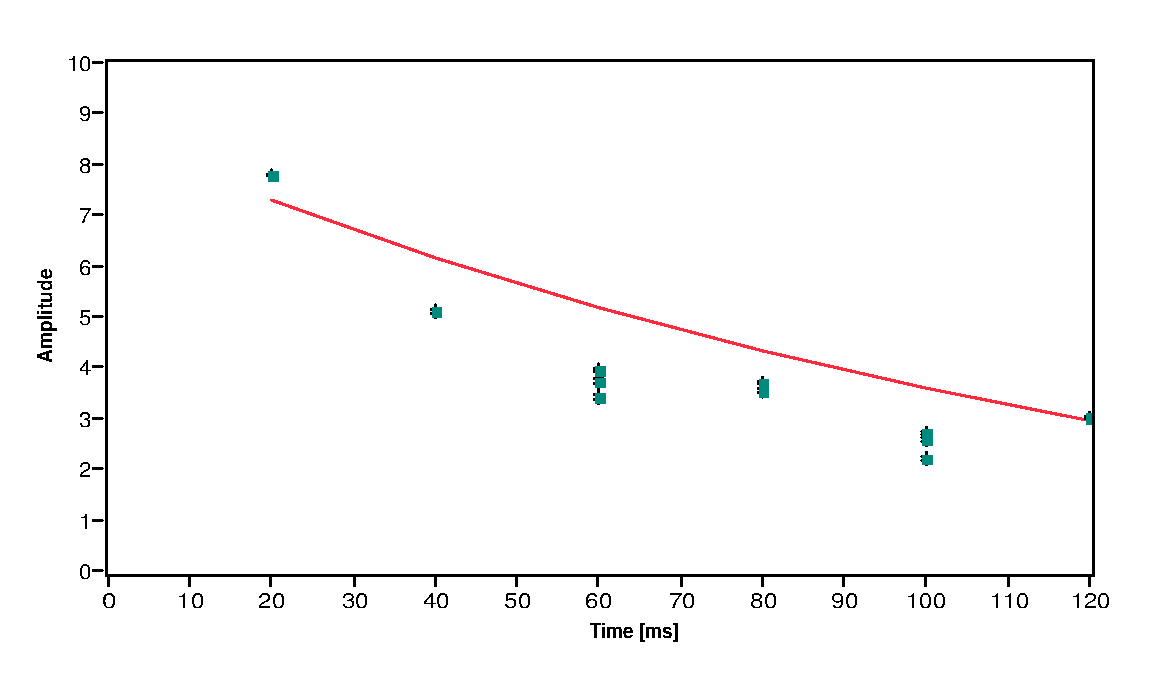
\includegraphics[width=70mm]{./Resources/t2_meas_p1.eps}
			\caption{T2-Messung Probe 1 mit Fit.}
			\label{fig:t2_p1}
		\end{figure}
	\end{minipage}
	\hfill
	\begin{minipage}[t]{0.45\textwidth}
		\centering
		\begin{figure}
			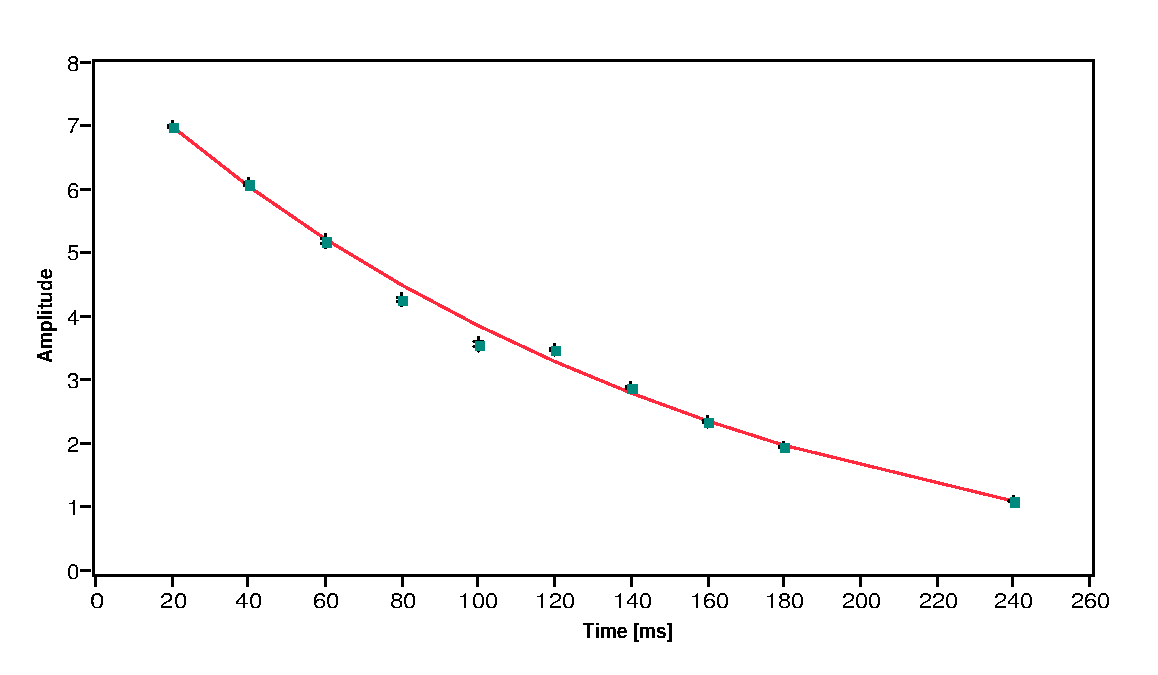
\includegraphics[width=70mm]{./Resources/t2_meas_p3.eps}
			\caption{T2-Messung Probe 3 mit Fit.}
			\label{fig:t2_p3}
		\end{figure}
	\end{minipage}
\end{frame}

\begin{frame}
	\frametitle{$T_2$-Measurement: Carr-Purcell Sequence}
	\textbf{Improve dephasing problem of spin-echo method:}
	\begin{itemize}
		\item Inject a $180^\circ$-Pulse on odd multiples of a time $\tau$.
		\item The system is phase coherent on even multiples of a time $\tau$.
	\end{itemize}
	\begin{minipage}[t]{0.45\textwidth}
		\centering
		\begin{figure}
			\includegraphics[width=60mm]{./Resources/t2_p1_cp.eps}
			\caption{T2-Messung über Carr-Purcell Probe 1 mit Fit.}
			\label{fig:t2_p1_cp}
		\end{figure}
	\end{minipage}
	\hfill
	\begin{minipage}[t]{0.45\textwidth}
		\centering
		\begin{figure}
			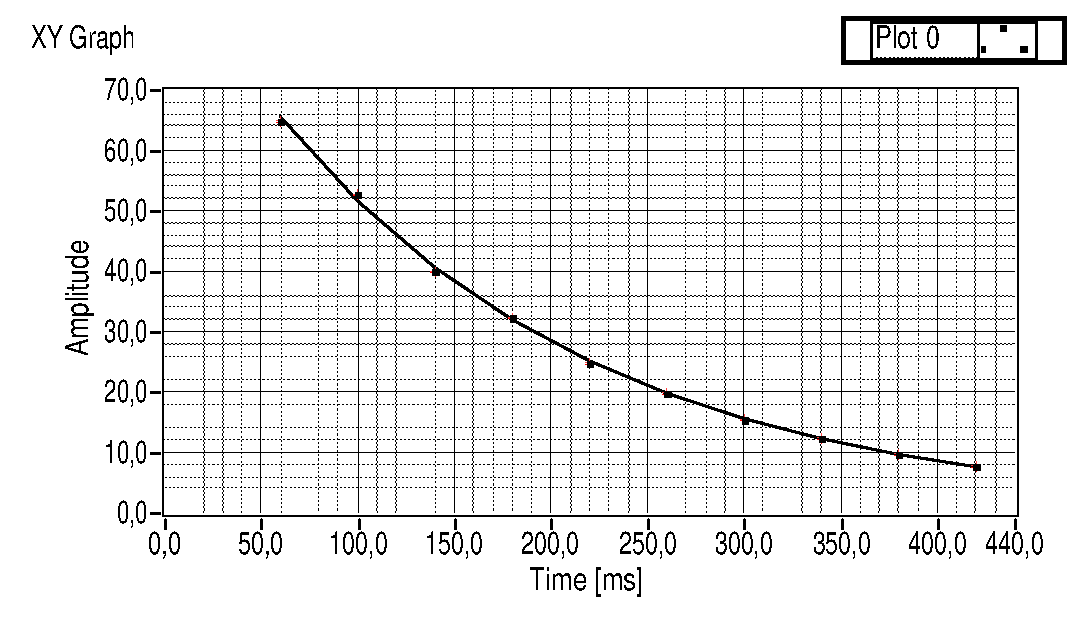
\includegraphics[width=60mm]{./Resources/t2_p3_cp.eps}
			\caption{T2-Messung über Carr-Purcell Probe 3 mit Fit.}
			\label{fig:t2_p3_cp}
		\end{figure}
	\end{minipage}
\end{frame}

\begin{frame}
	\frametitle{$T_1$-Measurement: Spin Echo}
	\textbf{Spin-Echo, but start with a $180^\circ$-Pulse (Anti-parallel Magnetization)}
	\begin{minipage}[t]{0.45\textwidth}
		\centering
		\begin{figure}
			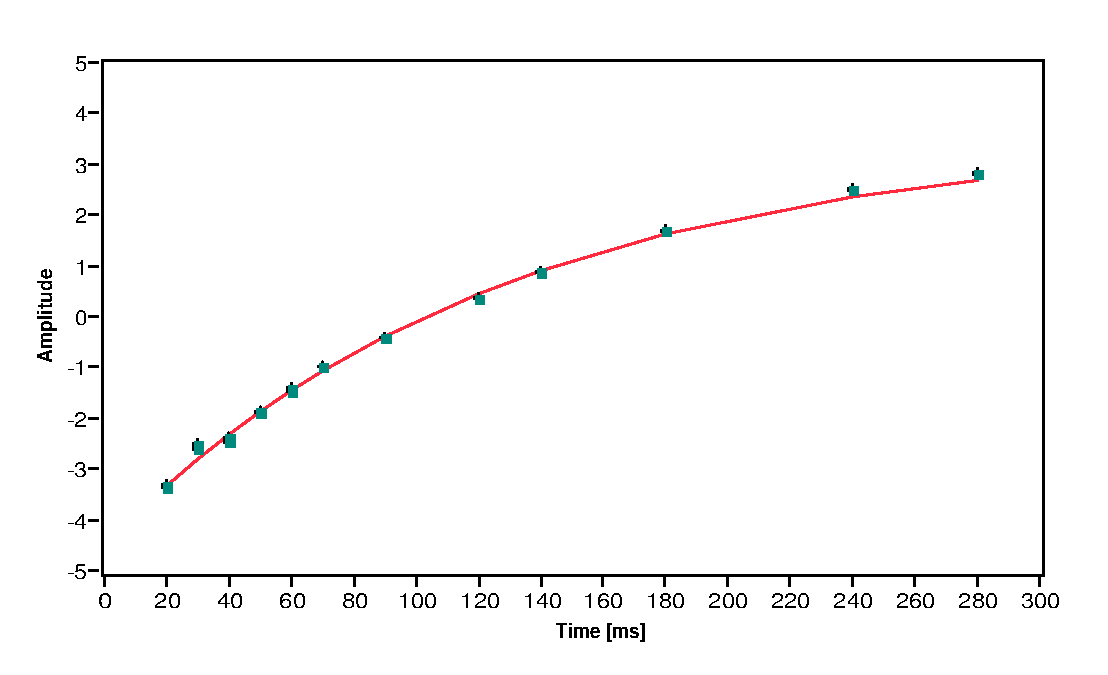
\includegraphics[width=70mm]{./Resources/t1_meas_p1.eps}
			\caption{T1-Messung Probe 1 mit Fit.}
			\label{fig:t1_p1}
		\end{figure}
	\end{minipage}
	\hfill
	\begin{minipage}[t]{0.45\textwidth}
		\centering
		\begin{figure}
			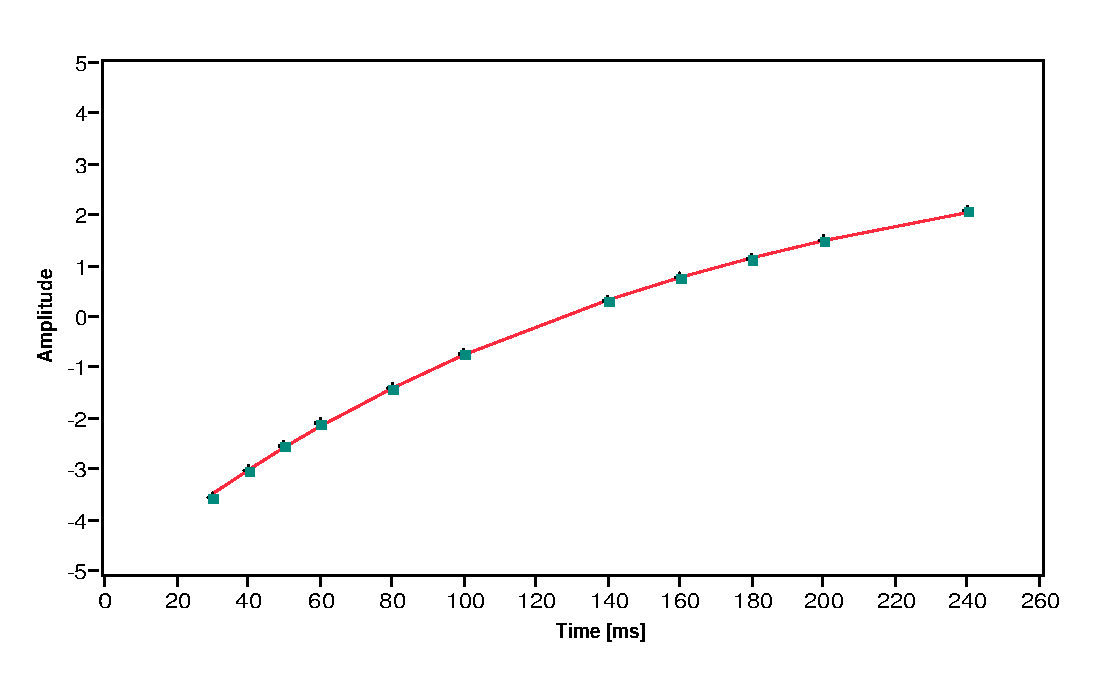
\includegraphics[width=70mm]{./Resources/t1_meas_p3.eps}
			\caption{T1-Messung Probe 3 mit Fit.}
			\label{fig:t1_p3}
		\end{figure}
	\end{minipage}
\end{frame}

\begin{frame}
	\frametitle{Relaxation Times: Evaluation}
	\begin{table}[H] 
		\centering
		\caption{Relaxation times: Measured values}
		\label{tab:relaxtimes}
		\begin{tabular}{cccc}
			\toprule
			Zeit & $T_1$ [$\mathrm{ms}$] & $T_2$ [$\mathrm{ms}$] & $T_2$ [$\mathrm{ms}$]\\
			Methode & Spin-Echo & Spin-Echo & Carr-Purcell\\
			\midrule
			Probe 1 (Gd 1:500)& $\err{125,5}{0,6}$ & $\err{119,5}{0,5}$ & $\err{140,1}{0,4}$\\
			Probe 3 (Gd 1:600)& $\err{150,5}{1,2}$ & $\err{139,3}{0,8}$ & $\err{166,9}{0,4}$\\
			\bottomrule
		\end{tabular}
	\end{table}
	
\end{frame}

\end{document}

\section{Introduction}

\begin{frame}
  \frametitle{Introduction}
  
    \textbf{What is lasercooling?}
    \begin{itemize}
    \item technique for cooling atomic or molecular samples
    \item down to 100 $\mu K$
    \item exchange of momentum between atoms and optical field
    \end{itemize}
    
    \pause  
    \bigskip
    \textbf{What is it used for?}
    \begin{itemize}
      \item high resolution spectroscopy
      \item Bose-Einstein condensate
      \item recently: cooling of molecules
      \begin{itemize}
        \item cold chemistry
        \item astrochemistry
      \end{itemize}
    \end{itemize}
  
\end{frame}

\section{Theoretical Background}

\subsection{Temperature}

\begin{frame}
  \frametitle{Temperature}
  \begin{columns}
    \column{.5\textwidth}
      \textbf{Thermodynamics:}
      \begin{itemize}
        \item parameter of state of a closed system
        \item in thermal equilibrium with its surroundings
      \end{itemize}
    \column{.5\textwidth}
      \pause
      \textbf{here:}
      \begin{itemize}
        \item describes the average kinetic energy
        \item Maxwell-Boltzmann velocity distribution
        \item per d.o.f.: $\langle E_{kin} \rangle = \frac{1}{2} k_B T$
        
      \end{itemize}
  \end{columns}
\end{frame}

\subsection{Entropy}

\begin{frame}
  \frametitle{Entropy}
  \begin{center}
    \textbf{Entropy:} $dS = \frac{\delta Q}{T}$ %, $S = k_b ln(\Omega)$
  \end{center}
  \begin{block}{2nd law of thermodynamics:}
    The sum of the entropies of all participating bodies is increased.    
  \end{block}
    \pause
    \bigskip
    \alert{Laser cooling in conflict with 2nd law?}
    
    \bigskip
    \pause
    $\Rightarrow$ Atoms don't form a closed system.
    \begin{itemize}
      \item \textbf{atoms} lose entropy
      \item \textbf{light field}  gains entropy
    \end{itemize}
    
    \medskip
      
\end{frame}

\subsection{Optical Forces on Neutral Atoms}

\begin{frame}
  \frametitle{Absorbtion}

  
  \begin{columns}
    \column{.5\textwidth}
      \begin{itemize}[<+->]
        \item well defined hyperfine state transition
        \item Absorption of photon with momentum $p = \hbar \omega / c = \hbar k$ 
        \item transition to excited state
        \item decay to ground state:
          \begin{itemize}
            \item<4-> \textbf{spontaneous} emission
            \item<4-> \textbf{stimulated} emission   
        \end{itemize}
      \end{itemize}
       
    \column{.5\textwidth}
    \begin{figure}
      \centering
      \includegraphics[scale=1]{Rb85_spek.png}
      \caption{D2-Line of $\mathrm{^{85} Rb}, \lambda = 780$nm [1]}
      \label{fig:D2-line}
    \end{figure}
    
  \end{columns}
  
\end{frame}



\begin{frame}
  \frametitle{Spontaneous vs. Stimulated Emission}
  \begin{columns}
    \column{.5\textwidth}
    \begin{figure}
      \centering
      \includegraphics[scale=0.07]{spon.JPG}
      \caption{Spontaneous emission of a photon [2]}
      \label{fig:spon-em}
    \end{figure}
    \vspace{-0.7cm}
    \begin{itemize}
      \item characterized by natural decay rate $\gamma = 1/\tau$      
      \item random direction
      \only<3->{
      \item on average: effect of spon. em. \alert{cancels out}}
    \end{itemize}
    \visible<2>{\centering
    \includegraphics[scale=0.04]{Random.JPG}}    
    \column{.5\textwidth}
    \visible<4->{
    \vspace{-1.8cm}
    \begin{figure}
      \centering
      \includegraphics[scale=0.07]{stim.JPG}
      \caption{Stimulated emission [2]}
      \label{fig:stim-em}
    \end{figure}
    \begin{itemize}
      \item influenced by photon of the same energy
      \item same direction and phase
      \item \alert{net transfer of zero momentum}, no cooling
    \end{itemize} }  
    
  \end{columns}
\end{frame}

\begin{frame}
  \frametitle{Radiative Optical Forces}
     \begin{center}
       \textbf{Absorption of a photon:}
     
       \medskip     
       {\Large $\vec{F} = \frac{d\vec{p}}{dt} = \hbar \vec{k} \gamma_p $} \quad with \qquad {\Large $\gamma_p=\frac{s_0\gamma/2}{1+s_0+[2(\delta+\omega_D)/\gamma]^2}$}
     
       \smallskip
     \end{center}
     
     \begin{columns}
       \column{.5\textwidth}
         \begin{itemize}
           \item ratio $s_0=I/I_s$ intensity to saturation intensity
           \item decay rate $\gamma = 1/\tau$
         \end{itemize}
         \visible<2->{\begin{figure}
           \centering
           \includegraphics[scale=0.06]{Doppler1.JPG}
         \end{figure}}
       \column{.5\textwidth}
         \begin{itemize}
           \item Doppler shift $\omega_D = -\vec{k} \cdot \vec{v}$
           \item Laser detuning $\delta \equiv \omega_l - \omega_a$
         \end{itemize}
         \medskip
         \visible<2->{\begin{figure}
           \centering
           \includegraphics[scale=0.06]{Doppler2.JPG}
         \end{figure}}
           
     \end{columns} 
\end{frame}

\subsection{Doppler Limit}
\begin{frame}
  \frametitle{Doppler Limit}
  \begin{itemize}
    \item average momentum transfer zero
    \item but \alert{rms scatter is finite!}
    \item random walk in space 
    \item<2-> diffusion in momentum space with $D_0 \equiv \frac{2(\Delta p)^2}{\Delta T} = 4 \gamma_p(\hbar\gamma)^2$. 
    \item<2-> In steady state we have: $T_D = \frac{\hbar\gamma }{2 k_B}$
  \end{itemize}
\end{frame}

\section{Slowing atoms}

\subsection{Zeeman Slower}

\begin{frame}
  \frametitle{Zeeman Slower}
  \begin{figure}
    \centering
    \includegraphics[scale=0.6]{Zeeman-Slower.png}
    \caption{Apparatus for beam slowing [3]}
  \end{figure}
\end{frame}

\begin{frame}
  \frametitle{Zeeman Slower (2)}
  \begin{columns}
  \column{.5\textwidth}
    \begin{figure}
      \centering
      \includegraphics[scale=1]{Zeeman-Solenoid.JPG}
      \caption{real solenoid for Zeeman slowing on an optical table [4]}
    \end{figure} 
   \column{.5\textwidth}
     {\Large $\gamma_p=\frac{s_0\gamma/2}{1+s_0+[2(\delta+\omega_D)/\gamma]^2}$}
     
     \medskip
     
     Adjustment of the right frequency:
     \pause
     \medskip 
     \begin{block}{Zeeman effect}
       Zeeman effect on hyperfine structure: $ \Delta E = g_j \mu_b m_j B$
       \smallskip
       
       $\Rightarrow$ detuning of transition: $\delta_{Ze} = \frac{\mu_B}{\hbar} (m^{(2)}_j g^{(2)}_j - m^{(1)}_j g^{(1)}_j) B(z) $
     \end{block}
     
  \end{columns}
\end{frame}

\begin{frame}
  \frametitle{Zeeman Slower (3)}
  \begin{columns}
  \column{.5\textwidth}
    \begin{figure}
      \centering
      \includegraphics[scale=1]{Rb85_spek.png}
      \caption{repumping, for comparison \textcolor{blue}{$\nu_{D2} = 385 THz$ }[1]}
    \end{figure} 
   \column{.5\textwidth} 
   \pause
     \textbf{Example Rubidium 85:}
     \begin{itemize}
       \item $T_{oven} = 570K$
       \item $\bar{v} = 402 m/s$
       \item $L_{min} = 0.75 m$
       \item $t_{min} = 3.72 ms$
       \item $T_D = 140 \mu K$
       \item $\bar{v}_D = 0.20 m/s$
     \end{itemize}
  \end{columns}
\end{frame}

\begin{frame}
  \frametitle{Zeeman Slower (4)}
  \begin{figure}
    \centering
    \includegraphics[scale=0.6]{Zeeman-Slower.png}
    \caption{Measuring the speed distribution of the atoms [3]}
  \end{figure}
\end{frame}

\subsection{Optical Molasses}

\begin{frame}
  \frametitle{Optical Molasses}
  \begin{columns}
  \column{.5\textwidth}
    \begin{itemize}
      \item two counterpropagating waves
      \item for small velocities: $\vec{F_{OM}} = - \beta \vec{v}$
      \item viscous damping: \textbf{"optical molasses"}
    \end{itemize}
    
   \column{.5\textwidth} 
     \begin{figure}
       \centering
       \includegraphics[scale=.5]{velocity-dependence.png}
       \caption{Velocity dependence of the optical damping forces [5]}
     \end{figure} 
  \end{columns}
\end{frame}

\section{Optical Traps}

\subsection{Magneto-optical Traps}

\begin{frame}
  \frametitle{Magneto-optical Trap (MOT)}
  \begin{columns}
  \column{.5\textwidth}
    \begin{itemize}
      \item \alert{Optical Molasses is not a trap!}
      \item velocity dependent and spatial dependent forces
    \end{itemize}
    
    \medskip
    \pause
    \begin{itemize}
      \item requires slow atoms
      \item linear gradient in B-field
      \item 3-dim optical molasses
    \end{itemize}       
    
   \column{.5\textwidth} 
     \begin{figure}
       \centering
       \includegraphics[scale=.3]{MOT-Foto.jpg}
       \caption{Photography of an Experiment with a MOT [6]}
     \end{figure} 
  \end{columns}
\end{frame}

\begin{frame}
  \frametitle{Magneto-optical Trap (2)}
  \begin{columns}
  \column{.5\textwidth}
     \begin{figure}
     \centering
     \includegraphics[scale=.3]{anti-helmholtz.png}
     \caption{Anti-Helmholtz coils produce a linearly inhomogeneous magnetic field [7]}    
     \end{figure}    
   \column{.5\textwidth} 
   \pause
   \textbf{Influence of polarisation of photons on optical transitions}
   \begin{itemize}
     \item $\sigma^+$ - polarisation: photon has spin $+ \hbar \Rightarrow \Delta m=+1$
     \item $\sigma^-$ - polarisation: photon has spin $- \hbar \Rightarrow \Delta m=-1$
   \end{itemize}
     
  \end{columns}
  
\end{frame}

\begin{frame}
  \frametitle{Magneto-optical Trap (3)}
  \begin{figure}
    \centering
    \includegraphics[scale=1.5]{Mot_posforce.png}
    \caption{functionality of a MOT in 1-D. [8]}
  \end{figure}
\end{frame}

\begin{frame}
  \frametitle{Conclusion}
  \begin{itemize}
  \item momentum $\hbar \vec{k}$ of a photon is used to slow down atoms
  \item only spontaneous emission contributes to cooling process
  \item \textbf{Zeeman slower} uses Zeeman effect to decelerate atoms from high tempereatures to very low ones
  \item \textbf{optical molasses}: counter propagating laser beams produce a damping force
  \item \textbf{magneto-optical}: For trapping neutral atoms we need velocity and spatial dependent forces
  %\item cooling below the Doppler Limit: ''Sisyphus laser cooling''
  \end{itemize}
\end{frame}

\begin{frame}
  \begin{center}
    {\Huge Thank you for your attention.}
  \end{center}

\end{frame}

\begin{frame}
  \frametitle{Sources}
  {\small
  \begin{itemize}
    \item Metcalf, H.J., van der Straten, P., Laser Cooling and Trapping. New York: Springer-Verlag 1999
    \item Demtröder, W., Experimentalphysik 3 - Atome, Moleküle und Festkörper. Heidelberg: Springer-Verlag 2010
    \item Harris, R., Moderne Physik, München: Pearson-Verlag 2013
    \item A.K. Hansen et al., Efficient rotational cooling of Coulomb-crystallized
molecular ions by a helium buffer gas, Nature, Vol 508, page 76, 2014
    \item Laserkühlung - Wikipedia, \url{https://de.wikipedia.org/wiki/Laserk\%C3\%BChlung} (18.05.2016)
    \item Zeeman-Slower - Wikipedia, \url{https://de.wikipedia.org/wiki/Zeeman-Slower} (20.05.2016)
    \item Magneto-optische Falle - Wikipedia, \url{https://de.wikipedia.org/wiki/Magneto-optische_Falle} (21.05.2016)
    \item Sysiphuskühlung - Wikipedia, \url{https://de.wikipedia.org/wiki/Sisyphusk\%C3\%BChlung} (21.05.2016)
  \end{itemize}
  }
\end{frame}

\begin{frame}
  \frametitle{Sources of the Pictures}
     {\small
     [1] Von Jkrieger 15:39, 19. Jun 2005 (CEST) - selbst gezeichnet, Bild-frei, \url{https://de.wikipedia.org/w/index.php?curid=752880} 
      
     [2] Harris, R., Moderne Physik, München: Pearson-Verlag 2013, page 536
     
     [3] Metcalf, H.J., van der Straten, P., Laser Cooling and Trapping. New York: Springer-Verlag 1999, page 9
     
     [4] Von KaiMartin - Eigenes Werk, CC BY-SA 3.0, \url{https://commons.wikimedia.org/w/index.php?curid=22575450}
     
     [5] Metcalf, H.J., van der Straten, P., Laser Cooling and Trapping. New York: Springer-Verlag 1999, page 9
     
     [6] Welt der Physik - \url{http://www.weltderphysik.de/uploads/tx_wdpcrop/1120130920_MOTDespec_Dwight_Whitaker.jpg} (19.05.2016)
     
     [7] Metcalf, H.J., van der Straten, P., Laser Cooling and Trapping. New York: Springer-Verlag 1999, page 21
     
     [8] Von Martin Horbanski, --Jkrieger 10:20, 20. Jun 2005 (CEST) - selbst gezeichnet, Bild-frei, \url{https://de.wikipedia.org/w/index.php?curid=754089}
     
     }
     
\end{frame}

%\begin{frame}
%  \begin{itemize}
%    \item \url{https://de.wikipedia.org/wiki/LaserkC3BChlung}
%    \item \url{http://scienceblogs.com/principles/files/2013/08/Sisyphus-big.jpg}
%    \item \url{http://www.weltderphysik.de/uploads/tx_wdpcrop/1120130920_MOTDespec_Dwight_Whitaker.jpg}
%    \item \url{https://upload.wikimedia.org/wikipedia/de/0/00/Mot_posforce.png}
%  \end{itemize}
%\end{frame}
%
%\begin{frame}
%  \frametitle{Phase Space Density}
%  \begin{block}{Liouville Theorem}
%     Phase space density $\rho( \vec{r}, \vec{p}, t)$ is constant along the trajectories of the system by using conservative forces.
%  \end{block}
%  
%  \medskip
%  
%  $\Rightarrow$ Increasing $\rho$ requires non-conservative forces, 
%  
%  i.e. \textbf{velocity-dependent forces}
%  
%  \medskip
%  
%  $\Rightarrow$ \textbf{spontaneous emission}
%  
%\end{frame}


\end{document}